\documentclass[11pt]{article}
\usepackage[title]{appendix}
\usepackage{amsmath,amssymb,amsthm}
\usepackage{enumitem}
\usepackage[left=1in,right=1in,top=1in,bottom=1in]{geometry}
\usepackage{tikz}
\usetikzlibrary{cd,decorations.pathmorphing}
\usepackage{xcolor}
\usepackage{sectsty,wrapfig}
\usepackage{hyperref}


\newtheorem{thm}{Theorem}[section]
\newtheorem{prp}[thm]{Proposition}
\newtheorem{lmm}[thm]{Lemma}
\newtheorem{crl}[thm]{Corollary}
\newtheorem{ques}[thm]{Question}
\newtheorem{fact}[thm]{Fact}

\theoremstyle{definition}
\newtheorem{dfn}[thm]{Definition}
\newtheorem{eg}[thm]{Example}

\theoremstyle{remark}
\newtheorem{rmk}[thm]{Remark}

\def\wt#1{\widetilde{#1}}
\def\ov#1{\overline{#1}}
\def\mr#1{{\mathring{#1}}}

\def\sgray{{\textnormal{gray}}}
\def\sred{{\textnormal{red}}}
\def\syellow{{\textnormal{yellow}}}
\def\sorange{{\textnormal{orange}}}
\def\sblue{{\textnormal{blue}}}


\def\Z{\mathbb{Z}}
\def\C{\mathbb{C}}
\def\P{\mathbb{P}}
\def\R{\mathbb{R}}
\def\Q{\mathbb{Q}}
\def\D{\mathbb{D}}
\def\M{\mathfrak{M}}
\def\cA{\mathcal{A}}
\def\cD{\mathcal{D}}
\def\cG{\mathcal{G}}
\def\cI{\mathcal{I}}
\def\cM{\mathcal{M}}
\def\cT{\mathcal{T}}
\def\cN{\mathcal{N}}
\def\cP{\mathcal{P}}
\def\cU{\mathcal{U}}
\def\rI{{\mathring{I}}}

\def\cmt#1{\textcolor{purple}{(#1)}}
\def\tn#1{\textnormal{#1}}
\def\pr{{\textnormal{pr}}}


\begin{document}

\setlength{\parskip}{\baselineskip}
\setlength{\parindent}{0cm}

\section{Introduction}

.....(introduction)

{\bf Define the kind of bundle we work with in this paper:}
Given a smooth homology sphere $M$, define a {\it framed $(M,\infty)$-bundle} $(\pi:E\to B,\sigma, \tau, F)$ (abbreviate all these to $\pi$) to be a smooth fiber bundle $\pi:E\to B$ with fiber $M$, with a smooth section $\sigma$, a trivialization $\tau$ of the bundle near $\sigma$, and a smooth vertical framing $F$ of $\pi$ ``standard'' near $\sigma$. 

{\bf Define the bracket operation, $\pi_1,\pi_2\to[\pi_1,\pi_2]$ on such bundles, in an intuitively clear but not necessarily rigorous way.}

{\bf Define cobracket and coproduct on graph cohomology (everything is over $\Q$):}
\begin{itemize}
\item First, define the graph complex $\cG'$---the $\Q$-vector space spanned by (with correct orientation definition, omitted here) connected graphs containing either a univalent vertex or a simple loop (an edge starting and ending at the same vertex). 
The coboundary operation $\delta$ is given by contracting an edge. 
In $\delta$ and all the operations on graphs below, whenever a graph not in $\cG'$ appears (a graph that has a univalent vertex or simple loop), we set it to 0. 
\item Taking the homology of $\cG'$ with respect to $\delta$, denote by $H^*{\cG'}$. 

\item Define the cobracket operation to be the linear map
\begin{align*}
\Delta_{[,]}: \cG'&\longrightarrow\cG'\otimes\cG'\\
\Gamma&\longrightarrow \sum_{\Gamma'\le\Gamma}\big(\Gamma'\otimes\Gamma/\Gamma'+(-1)^{..}\Gamma/\Gamma'\otimes\Gamma'\big), 
\end{align*}
where $\Gamma'$ ranges through all full subgraphs of $\Gamma$ that is connected, with no univalent vertex or simple loop.
\item Check that $\Delta_{[,]}$ commutes with $\delta$ and $\delta\otimes\tn{id}\pm\tn{id}\otimes\delta$, so it descends to 
$$\Delta_{[,]}: H^*{\cG'}\longrightarrow H^*(\cG'\otimes\cG')\approx H^*{\cG'}\otimes H^*{\cG'}.$$

\item Finally we also define the coproduct operation on $\cG'$ (this makes more sense for disconnected graphs but w=for connected graphs it is extra simple):  
\begin{align*}
\Delta_{\cdot}: \cG'&\longrightarrow \cG'\otimes\cG'\\
\Gamma&\longrightarrow \Gamma\otimes \tn{(the empty graph)} + \tn{(the empty graph)}\otimes\Gamma.
\end{align*}

\end{itemize}

{\bf Brief introduction to Kontsevich's characteristic classes.}
Given a framed $(M,\infty)$-bundle $\pi:E\to B$ as above, denote by  
$$K_\pi: H^*(\cG')\longrightarrow H^*(B)$$
Kontsevich's characteristic classes of $\pi$. 


\begin{thm}\label{formula_thm}
Suppose $d\ge3$. 
For $i=1,2$, suppose $M_i$ is a $d$-dimensional smooth homology sphere and 
suppose $\pi_i: E_i\to B_i$ is a framed $(M,\infty)$-bundle. 
(Now, $[\pi_1,\pi_2]: E\to S^d\times B_1\times B_2$ is the bracket bundle.)
Then, for all $\eta\in H^*\cG'$, 
\begin{align*}
K_{[\pi_1,\pi_2]}(\eta)=
\tn{PD}_{S^d}[S^d]\otimes
(K_{\pi_1}\otimes K_{\pi_2})(\Delta_{[,]}(\eta))
+\tn{PD}_{S^d}[pt]\otimes
(K_{\pi_1}\otimes K_{\pi_2})(\Delta_\cdot(\eta)).
\end{align*}
(Both LHS and RHS lives in 
$$H^*(S^d\times B_1\times B_2)\approx H^*(S^d)\otimes H^*(B_1)\otimes H^*(B_2).$$
$\tn{PD}_{S^d}$ means Poincar\'e dual on $S^d$; $[S^d]$ stands for the fundamental class of $S^d$ and $[pt]$ stands for the point class of $S^d$.)
\end{thm}


......(Then talk about the $(d+1)$-fold loop space structure on $\tn{BDiff}^{\tn{fr}}_\partial(D^d)$ and the theorem/corollary that it doesn't extend.)

(Below is an outline of the proof of Theorem \ref{formula_thm}.
Throughout, $\pi_1,\pi_2$ are given and fixed. 
)

\section{Conftilde}\label{conftilde_sec}

Construct the big configuration space $\widetilde{C}_A$. 
Show that it is a smooth manifold with boundary and corners. 
(These are mostly already written in the file ``conftilde'' I sent a while ago.)

What we need are the following: 

\begin{itemize}
\item $\widetilde{C}_A$ is a smooth manifold with boundary and corners; 
\item each $S_T$ is a stratum of $\widetilde{C}_A$; 
\item $\overline{S}_T=\bigsqcup_{T'}S_{T'}$, where the disjoint union is taken over all $A$-labeled trees $T'$ such that $T$ can be obtained from $T'$ by contracting some edges. 

\end{itemize}

Here is a schematic picture of $\wt{C}_A$ (the marked points are not drawn; the actual stratification structure of $\wt{C}_A$ is more complicated than what is shown in the picture): 

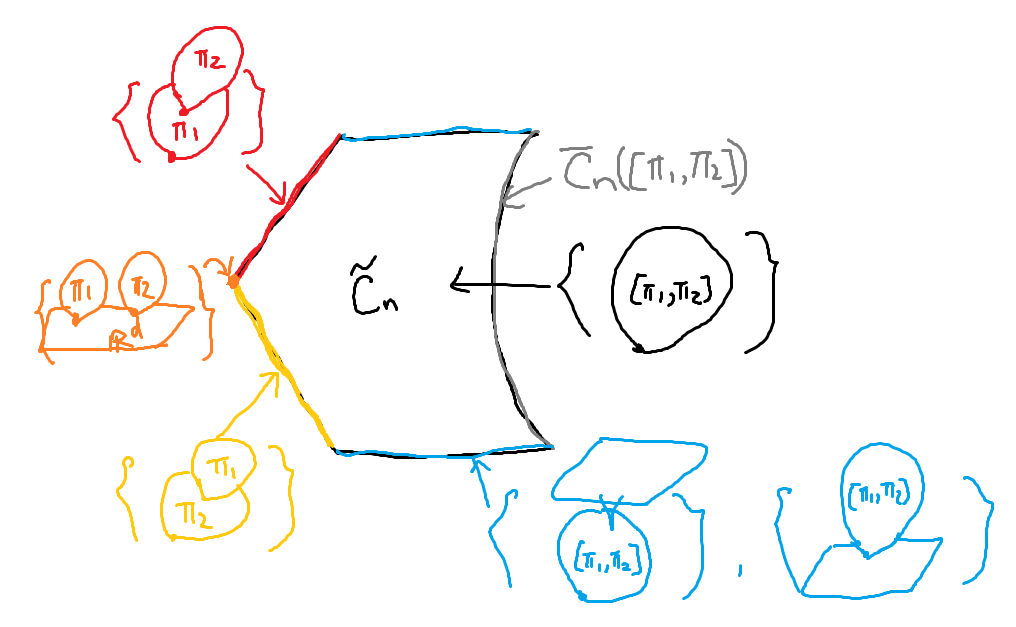
\includegraphics[scale=0.7]{conftilde.png}

The boundary of $\wt{C}_A$ consists of the following parts: 
\begin{itemize}
\item the gray part, denoted by $\ov{S}_\sgray$, is $\ov{C}_A([\pi_1,\pi_2])$; its interior, denoted by $S_\sgray$, is $C_A([\pi_1,\pi_2])$; 
\item ${S}_\sblue:=\bigcup_{T\in\cT_\sblue}S_T$, where $\cT_\sblue$ is the set of all $A$-labeled trees whose shape and space labels are like
$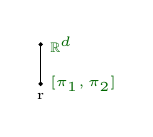
\begin{tikzpicture}
\node [below] at (0,0) {\tiny{r}};  
\node [right, black!60!green] at (0,0) {\tiny{$[\pi_1,\pi_2]$}};
\node [right, black!60!green] at (0,0.5) {\tiny{$\R^d$}};
\draw [fill] (0,0) circle [radius=0.02];
\draw [fill] (0,0.5) circle [radius=0.02];
\draw (0,0) -- (0,0.5);
\end{tikzpicture}$ or 
$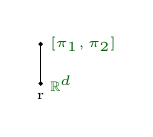
\begin{tikzpicture}
\node [below] at (0,0) {\tiny{r}};  
\node [right, black!60!green] at (0,0) {\tiny{$\R^d$}};
\node [right, black!60!green] at (0,0.5) {\tiny{$[\pi_1,\pi_2]$}};
\draw [fill] (0,0) circle [radius=0.02];
\draw [fill] (0,0.5) circle [radius=0.02];
\draw (0,0) -- (0,0.5);
\end{tikzpicture}$;
and let $\ov{S}_\sblue$ be the closure of $S_\sblue$;
\item ${S}_\sred:=\bigcup_{T\in\cT_\sred}S_T$, where $\cT_\sred$ is the set of all $A$-labeled trees with the following shape and space labels: 
$\begin{tikzpicture}
\node [below] at (0,0) {\tiny{r}};  
\node [right, black!60!green] at (0,0) {\tiny{$\pi_1$}};
\node [right, black!60!green] at (0,0.5) {\tiny{$\pi_2$}};
\draw [fill] (0,0) circle [radius=0.02];
\draw [fill] (0,0.5) circle [radius=0.02];
\draw (0,0) -- (0,0.5);
\end{tikzpicture}$;
and let $\ov{S}_\sred$ be the closure of $S_\sred$;
\item ${S}_\syellow:=\bigcup_{T\in\cT_\syellow}S_T$, where $\cT_\syellow$ is the set of all $A$-labeled trees with the following shape and space labels: 
$\begin{tikzpicture}
\node [below] at (0,0) {\tiny{r}};  
\node [right, black!60!green] at (0,0) {\tiny{$\pi_2$}};
\node [right, black!60!green] at (0,0.5) {\tiny{$\pi_1$}};
\draw [fill] (0,0) circle [radius=0.02];
\draw [fill] (0,0.5) circle [radius=0.02];
\draw (0,0) -- (0,0.5);
\end{tikzpicture}$;
and let $\ov{S}_\syellow$ be the closure of $S_\syellow$; 
\end{itemize}

We also define
${S}_\sorange:=\bigcup_{T\in\cT_\sorange}S_T$, where $\cT_\sorange$ is the set of all $A$-labeled trees with the following shape and space labels: 
$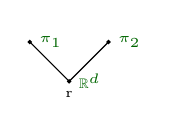
\begin{tikzpicture}
\node [below] at (0,0) {\tiny{r}};  
\node [right, black!60!green] at (0,0) {\tiny{$\R^d$}};
\node [right, black!60!green] at (-0.5,0.5) {\tiny{$\pi_1$}};
\node [right, black!60!green] at (0.5,0.5) {\tiny{$\pi_2$}};
\draw [fill] (0,0) circle [radius=0.02];
\draw [fill] (-0.5,0.5) circle [radius=0.02];
\draw [fill] (0.5,0.5) circle [radius=0.02];
\draw (-0.5,0.5) -- (0,0) -- (0.5,0.5);
\end{tikzpicture}$;
and let $\ov{S}_\sorange$ be the closure of $S_\sorange$. Then, $\ov{S}_\sorange=\ov{S}_\sred\cap\ov{S}_\syellow$. 

We define $\ov{C}^*_A=\ov{S}_\sred\cup\ov{S}_\syellow$.

% note that 
%${S}_T$ is a 1-parameter family of $\partial \ov{C}_n([\pi_1,\pi_2])$---its interior is diffeomorphic to 
%$$\partial \ov{C}_n([\pi_1,\pi_2])\times (0,1);$$

\section{Propagators}

Fix a volume form $\omega_0$ on $S^{d-1}$. 
For $i=1,2$, fix a propagator $\omega_i$ on $\ov{C}_2(\pi_i)$ such that on $\partial\ov{C}_2(\pi_i)$, $\omega_i$ is given by $\omega_0$. 

\subsection{Propagator on confstar}

$\omega_1,\omega_2$ naturally induce a propagator $\omega_*$ on $\ov{C}^*_2$. On the main strata of $\ov{C}^*_2$, define $\omega_*$ as follows: 
\begin{itemize}
\item On the stratum $S_{11}$ consisting of  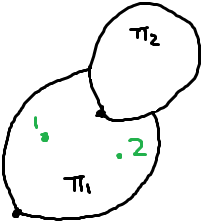
\includegraphics[scale=0.4]{mouse11}, 
there is the forgetful map
$f_{11}:S_{11}\to \ov{C}_2(\pi_1)$. We define $\omega_*|_{S_{11}}=f_{11}^*(\omega_1)$. 

\item On the stratum $S_{22}$ consisting of  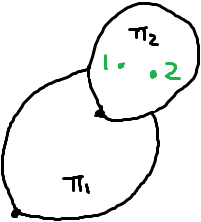
\includegraphics[scale=0.4]{mouse22}, 
there is the forgetful map
$f_{22}:S_{22}\to \ov{C}_2(\pi_2)$. We define $\omega_*|_{S_{22}}=f_{22}^*(\omega_2)$. 

\item On the stratum $S_{12}$ consisting of  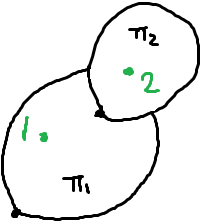
\includegraphics[scale=0.4]{mouse12}, 
there is the forgetful map
$f_{12}:S_{12}\to \ov{C}_2(\pi_1)$, where the second marked point is considered to be located at the node on $\pi_1$.  
We define $\omega_*|_{S_{22}}=f_{22}^*(\omega_2)$.

\item ...(There are 5 more situations, all variations of the above, permuting $\pi_1,\pi_2, 1,2$.) 
\end{itemize}

We then check that the above definitions are compatible when the main strata glue together. 
For example, the stratum $S'$ consisting of 
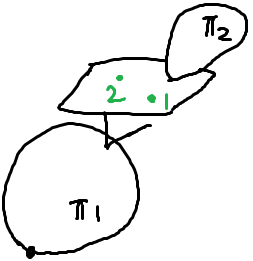
\includegraphics[scale=0.4]{S11capS22} lies in the intersection of $\ov{S}_{11}$ and $\ov{S}_{22}$;
but the $\omega_*$ constructed on $S_{11}$ and on $S_{22}$, when extended to here, agree, 
since they both become $(f')^*\omega_0$, where $f':S'\to S^{d-1}$ is the forgetful map recording the direction of the vector between the two points.

All other codimension-1 strata can be straight-forwardly checked like this as well. 
We may need to check higher-codimension strata as well but it shouldn't be hard.

%\begin{rmk}%not true and not needed anymore
%I lied a bit---``compatibility'' of $\omega_*$ along the gluing is a stronger condition then it is presented above. 
%Given two manifolds with boundary, $X,Y$, such that $\partial X\approx \partial Y=:W$, let $Z$ be the space obtained by gluing $X,Y$ together along their common boundary $W$, but we do not specify a smooth structure near $W$;
%then, say a form $\alpha$ on $X$ is compatible with a form $\beta$ on $Y$ if 
%\begin{itemize}
%\item $\alpha|_W=\beta|_{W}$;
%\item there are collar neighborhoods $N_X$ of $W$ in $X$ and $N_Y$ of $W$ in $Y$ (with projection maps $p_X:N_X\to W$, $p_Y:N_Y\to W$) such that 
%$\alpha|_{N_X}=p_X^*\alpha|_W$, $\beta|_{N_Y}=p_Y^*\beta|_W$. 
%\end{itemize} 
%The second condition says that in a collar neighborhood of the boundary the forms are trivial in the normal direction. 
%In our situation, this stronger compatibility condition should be achievable as well, if we impose a similar condition (``parallel to boundary'' near the boundary) on $\omega_1,\omega_2$. 
%\end{rmk} 

\subsection{Propagator on other parts of the boundary of conftilde}

To define a propagator on the blue part of $\partial\wt{C}_2$, we have no choice but to define it as induced from $\omega_0$ in the usual way. 

To define a propagator in the gray part of $\partial\wt{C}_2$, we just choose any propagator $\omega$ on $\wt{C}_2([\pi_1,\pi_2])$, so that $\omega|_{\partial\wt{C}_2([\pi_1,\pi_2])}$ is induced from $\omega_0$. 

Now we have defined a propagator on all of $\partial\wt{C}_2$. 

\subsection{Extend the propagator to the interior}


\begin{lmm}

\end{lmm}


To show that there exists a closed form on $\wt{C}_2$ extending the propagator we just defined on $\partial\wt{C}_2$, 
it suffices to show that the map 
$$H^{d-1}(\wt{C}_2)\xrightarrow{\tn{restriction}}H^{d-1}(\partial\wt{C}_2)$$
is surjective. 
It is therefore sufficient to show that $H^d(\wt{C}_2,\partial\wt{C}_2)=0$. But 
\begin{align*}
H^*(\wt{C}_2,\partial\wt{C}_2)\approx
H_{\dim(\wt{C}_2)-*}(\wt{C}_2-\partial\wt{C}_2)=
H_{\dim(\wt{C}_2)-*}\big(C_2([\pi_1,\pi_2])\times (0,1)\big)\\
\approx
H_{\dim(\wt{C}_2)-*}({C}_2([\pi_1,\pi_2]))
\approx H^{*-1}\big(\ov{C}_2([\pi_1,\pi_2]),\partial\ov{C}_2([\pi_1,\pi_2])\big), 
\end{align*}
%$\dim(\wt{C}_2)=\dim(C_2([\pi_1,\pi_2]))+1=3d+1+\dim(B_1)+\dim(B_2)$ 
and this is 0 when $*-1<d+1$; see the proof of Lemma 2.12 in \href{https://arxiv.org/pdf/2109.01609}{Watanabe's addendum paper}. 

We choose and fix such an extension. This gives us a propagator $\wt\omega$ on $\wt{C}_2$. 

\section{Configuration space integrals}

For simplicity here we will only sketch part of the proof of Theorem \ref{formula_thm}, namely we only justify the first term on the RHS. 
(The second term is slightly more complicated but not much: basically because we only work with the point class on $S^d$---it is only 0-dimensional so you can still easily achieve transversality as needed. The second term is not needed for the corollary about the loop space structure on $\tn{BDiff}^{\tn{fr}}_\partial(D^d)$ either.) 

Given a graph $G$, we denote by $V(G)$ its vertex set and $E(G)$ its edge set. 

Suppose $\Gamma$ is a cocycle in graph cohomology. (For the simplicity of notation we assume $\Gamma$ is one graph---when it is a formal sum everything works as well.)

For every edge $e$ of $\Gamma$, we have the forgetful map 
$$f_e:\wt{C}_{V(\Gamma)}\longrightarrow\wt{C}_2.$$
And, when restricted to the gray (resp. red, orange, and yellow) part of $\partial\wt{C}_{V(\Gamma)}$, it is the forgetful map
$$f_e:\ov{C}_{V(\Gamma)}([\pi_1,\pi_2])\longrightarrow\ov{C}_2([\pi_1,\pi_2]) \qquad (\tn{resp. } f_e:\ov{C}^*_{V(\Gamma)}\longrightarrow\ov{C}^*_2).$$
Now we have the form $\bigwedge_{e\in E(\Gamma)}f_e^*\wt{\omega}$ on $\wt{C}_{V(\Gamma)}$. 
When restricted to the gray part of $\partial\wt{C}_n$, it is used to define Kontsevich's classes for the bundle $[\pi_1,\pi_2]$. 

To compute the ($\tn{PD}_{S^d}[S^d]$)-part of $K_{[\pi_1,\pi_2]}([\Gamma])$, we only need to compute, given arbitrary homology classes $\alpha_1\in H_*(B_1)$ and $\alpha_2\in H_*(B_2)$, the evaluation
$$\big\langle K_{[\pi_1,\pi_2]}([\Gamma]), [S^d]\otimes\alpha_1\otimes\alpha_2 \big\rangle.$$
For $i=1,2$, suppose $\alpha_i$ is represented by a sub-pseudo-manifold $\iota_i:B'_i\hookrightarrow B_i$. (For simplicity you can think of a smooth submanifold instead.)

For any $n$: notice that the projection map 
$\wt{p}:\wt{C}_n\to B_1\times B_2$
is a fiber bundle, and so is the restriction of $\wt{p}$ to each stratum of $\wt{C}_n$.
Let us pull everything back along $(\iota_1,\iota_2)$, so that the base gets changed to $B'_1\times B'_2$ instead of $B_1\times B_2$. 
Abusing notation, we still denote by
$\wt{C}_n,\ov{C}_n([\pi_1,\pi_2]),\ov{C}^*_n$
their pull-backs. 

Now, we have 
\begin{equation}
\label{integral_eqn}
\big\langle K_{[\pi_1,\pi_2]}([\Gamma]), [S^d]\otimes\alpha_1\otimes\alpha_2 \big\rangle=
\int_{\ov{C}_{V(\Gamma)}([\pi_1,\pi_2])}\bigwedge_{e}f_e^*{\omega}=
\int_{\tn{gray part of }\partial\wt{C}_{V(\Gamma)}}\bigwedge_{e}f_e^*\wt{\omega}.
\end{equation}
By Stocks' Formula (and the fact that $\wt\omega$ is closed), 
$$\int_{\partial\wt{C}_{V(\Gamma)}}\bigwedge_{e}f_e^*\wt{\omega}=\int_{\wt{C}_{V(\Gamma)}}d\Big(\bigwedge_{e}f_e^*\wt{\omega}\Big)=0,$$
so, 
$$(\ref{integral_eqn})=\int_{\tn{blue part of }\partial\wt{C}_{V(\Gamma)}}\bigwedge_{e}f_e^*\wt{\omega}+\int_{\ov{C}^*_{V(\Gamma)}}\bigwedge_{e}f_e^*{\omega_*}.$$
Since $\Gamma$ is a cocycle in graph cohomology, the first term is 0 just like in the proof of the well-definedness of Kontsevich's classes, so
$$\big\langle K_{[\pi_1,\pi_2]}([\Gamma]), [S^d]\otimes\alpha_1\otimes\alpha_2 \big\rangle=
\int_{\ov{C}^*_{V(\Gamma)}}\bigwedge_{e}f_e^*{\omega_*}.$$

\section{Configuration space integral on confstar}

We continue with the notation from last section (in particular, everything is over $B'_1, B'_2$ instead of $B_1, B_2$). 

It remains to show that 
\begin{equation}\label{stardecompose_eqn}
\big\langle (K_{\pi_1}\otimes K_{\pi_2})(\Delta_{[,]}[\Gamma]), \alpha_1\otimes\alpha_2 \big\rangle=
\int_{\ov{C}^*_{V(\Gamma)}}\bigwedge_{e}f_e^*{\omega_*}. 
\end{equation}
For a graph $G$, we denote by $V(G)$ its vertex set and $E(G)$ its edge set. 
The LHS above equals to\footnote{
A little more argument needed for this claim, but it is true.} 
\begin{align*}
\sum_{\Gamma'\le\Gamma}
\Big(&\int_{\ov{C}_{V(\Gamma')}(\pi_1)}
\bigwedge_{e\in E(\Gamma')}f_e^*\omega_1\Big)
\cdot
\Big(\int_{\ov{C}_{V(\Gamma/\Gamma')}(\pi_2)}
\bigwedge_{e\in E(\Gamma/\Gamma')}f_e^*\omega_2\Big)\\
&\pm
\Big(\int_{\ov{C}_{V(\Gamma/\Gamma')}(\pi_1)}
\bigwedge_{e\in E(\Gamma/\Gamma')}f_e^*\omega_1\Big)
\cdot
\Big(\int_{\ov{C}_{V(\Gamma')}(\pi_2)}
\bigwedge_{e\in E(\Gamma')}f_e^*\omega_2\Big).
\end{align*}
To prove (\ref{stardecompose_eqn}), it suffices to show that 
\begin{equation}\label{yellow_eqn}
\sum_{\Gamma'\le\Gamma}
\Big(\int_{\ov{C}_{V(\Gamma')}(\pi_1)}
\bigwedge_{e\in E(\Gamma')}f_e^*\omega_1\Big)
\cdot
\Big(\int_{\ov{C}_{V(\Gamma/\Gamma')}(\pi_2)}
\bigwedge_{e\in E(\Gamma/\Gamma')}f_e^*\omega_2\Big)=
\int_{\tn{yellow part of }\ov{C}^*_{V(\Gamma)}}\bigwedge_{e\in E(\Gamma)}f_e^*{\omega_*}
\end{equation}
and 
\begin{equation}\label{red_eqn}
\sum_{\Gamma'\le\Gamma}
\Big(\int_{\ov{C}_{V(\Gamma/\Gamma')}(\pi_1)}
\bigwedge_{e\in E(\Gamma/\Gamma')}f_e^*\omega_1\Big)
\cdot
\Big(\int_{\ov{C}_{V(\Gamma')}(\pi_2)}
\bigwedge_{e\in E(\Gamma')}f_e^*\omega_2\Big)=
\int_{\tn{red part of }\ov{C}^*_{V(\Gamma)}}\bigwedge_{e\in E(\Gamma)}f_e^*{\omega_*};
\end{equation}
here the ``red'' and ``yellow'' refers to the $\wt{C}_n$ picture in Section \ref{conftilde_sec}. 
Below we only prove (\ref{yellow_eqn}) since (\ref{red_eqn}) is completely similar. 

The yellow part of $\ov{C}^*_{V(\Gamma)}$ is simply
$$\sum_{V_1,V_2:V_1\sqcup V_2=V(\Gamma)}
\ov{C}_{V_1}(\pi_1)\times\ov{C}_{V_2\sqcup\{\star\}}(\pi_2),
$$
where $\star$ records the position of the node on $\pi_2$.
Therefore, the RHS of (\ref{yellow_eqn}) is
$$\sum_{V_1,V_2:V_1\sqcup V_2=V(\Gamma)}
\int_{\ov{C}_{V_2\sqcup\{\star\}}(\pi_2)}\int_{\ov{C}_{V_1}(\pi_1)}
\bigwedge_{\begin{subarray}{c}e\in E(\Gamma)\\\tn{both endpoints of }e\tn{ are in }V_1\end{subarray}}f_e^*{\omega_*}\wedge
\bigwedge_{\begin{subarray}{c}e\in E(\Gamma)\\ \exists\tn{ endpoint of }e\tn{ in }V_2\end{subarray}}f_e^*{\omega_*}. 
$$ 
For $V_1\subset V(\Gamma)$, we denote by $\Gamma'(V_1)$ the subgraph of $\Gamma$ spanned by vertices in $V_1$. Then, by the way $\omega_*$ is constructed, and by Fubini's Theorem, 
the above equals to 
$$\sum_{V_1,V_2:V_1\sqcup V_2=V(\Gamma)}
\Big(\int_{\ov{C}_{V_1}(\pi_1)}
\bigwedge_{e\in E(\Gamma'(V_1))} 
f_e^*{\omega_1}\Big)
\cdot
\Big(\int_{\ov{C}_{V_2\sqcup\{\star\}}(\pi_2)}
\bigwedge_{e\in E(\Gamma/\Gamma'(V_1))}
f_e^*{\omega_2}\Big). 
$$ 
This proves (\ref{yellow_eqn}). 


\begin{appendices}
\section{Extending differential forms in a manifold with boundary and corners from boundary to interior}

Suppose $M$ is a manifold with boundary and corners. Let $\partial M$ denote the closed boundary of $M$, i.e.~the union of all non-top-dimensional strata. 
In this section we prove the following 
\begin{prp}
Suppose for each stratum $S\subset\partial M$ of $M$, $\omega_S$ is a closed differential form of degree $k$ on $\ov{S}$, such that, for each pair of strata $T\subset \ov{S} \subset\partial{M}$, $\omega_T=\omega_S|_{\ov{T}}$. 
Then, there exists an open neighborhood $U$ of $\partial M$ and a closed differential form $\omega$ on $U$ such that $\omega|_{\ov{S}}=\omega_S$ for all strata $S\subset\partial M$. 
\end{prp}

First we prove the statement locally, in $(\R^{\ge0})^d\times\R^{n-d}$, where $0\le d\le n$ and $0\le k\le n$ are integers. 
%In $(\R^{\ge0})^d\times\R^{n-d}$, we use variables $x_1,\ldots,x_n$ to denote the coordinates. 
%Given $I=\{i_1,\ldots,i_k\}\subset\{1,\ldots,n\}$ where $i_1<\ldots<i_k$, we use the abbreviate $$dx_I:=dx_{i_1}\wedge\ldots\wedge dx_{i_k}.$$ 
For $I\subset\{1,\ldots,d\}$, define $H_I:=\big\{(x_1,\ldots,x_n)\big|\,\forall i\in I, x_i=0\big\}\subset (\R^{\ge0})^d\times\R^{n-d}$. 
Write $H_i:=H_{\{i\}}$ and $H_{i,j}=H_{\{i,j\}}$. 
\begin{lmm}\label{localformpatching_lmm}
Suppose for each $1\le i\le d$, $\omega_i$ is a degree-$k$ differential form on $H_i$, such that, for all $1\le i,j\le d$, $\omega_i|_{H_{i,j}}=\omega_j|_{H_{i,j}}$. 
Then, there exists a degree-$k$ differential form $\omega$ on $(\R^{\ge0})^d\times\R^{n-d}$, such that, for all $1\le i\le d$, $\omega|_{H_i}=\omega_i$. 
Moreover, if all $\omega_i$ are closed, $\omega$ can be taken to be closed as well. 
\end{lmm}
\begin{proof}
From the condition $\omega_i|_{H_{i,j}}=\omega_j|_{H_{i,j}}$ it is clear that for any $I\subset\{1,\ldots,d\}$, the forms $\omega_i|_{H_I}$ are the same for all $i\in I$. We hence denote it by $\omega_I$, which is on $H_I$. %Also write $\omega_{i,j}:=\omega_{\{i,j\}}$. 
Let $$p_I:(\R^{\ge0})^d\times\R^{n-d}\longrightarrow H_I$$
be the projection map, sending all $I$-coordinates to 0 and not changing the other coordinates. 
We take $\omega$ to be the alternating sum
$$
\omega=\sum_{1\le i\le d}p_{\{i\}}^*\omega_i
-\sum_{1\le i<j\le d}p_{\{i,j\}}^*\omega_{\{i,j\}}
+\sum_{1\le i<j<k\le d}p_{\{i,j,k\}}^*\omega_{\{i,j,k\}}
-\ldots+(-1)^{d-1}p_{\{1,\ldots,d\}}^*\omega_{\{1,\ldots,d\}}.
$$
To see that $\omega|_{H_i}=\omega_i$ for a given $i\in\{1,\ldots,d\}$, note that, for each $I\subset\{1,\ldots,d\}$ with $I\neq\emptyset$ and $i\notin I$,
$$(p_I^*\omega_I)|_{H_i}=p_I^*(\omega_I|_{H_i})=p_{I\sqcup\{i\}}^*(\omega_{I\sqcup\{i\}}|_{H_i})=(p_{I\sqcup\{i\}}^*\omega_{I\sqcup\{i\}})|_{H_i},$$ so these two terms cancel with each other. 
If all $\omega_i$s are closed, $\omega$ is clearly also closed. 
\end{proof}

Next, we patch the forms constructed locally to a global one. Without the closeness condition, this would be immediate by applying a partition of unity. With the closeness condition it is much subtler. 
The argument uses the same technique as translating between \v{C}ech and de Rham cohomology. 
Note that from now on, the index set $I$ has a different meaning than in Lemma \ref{localformpatching_lmm}. 

Given $p,q\in\Z^{\ge0}$, a manifold $M$ and a locally finite open cover $\cU=\{U_i\}_{i\in I}$ of $M$, recall a (skew-symmetric) $p$-\v{C}ech cochain of $q$-forms on $M$ is: for each sequence $(i_0,i_1,\ldots,i_p)\in I^{p+1}$, a differential $q$-form $\alpha_{i_0i_1\ldots i_p}$ on $\bigcap_{j=0}^pU_{i_j}$; such that for all $j$, 
$\alpha_{i_0\ldots i_ji_{j+1}\ldots i_p}=-\alpha_{i_0\ldots i_{j+1}i_j\ldots i_p}.$
We denote the $\R$-vector space of $p$-\v{C}ech cochain of $q$-forms on $M$ by $\check{C}^p_\cU(M;\cA^q)$. 
The \v{C}ech differential is 
\begin{align*}
&\check\delta:\check{C}^p_\cU(M;\cA^q)\longrightarrow\check{C}^{p+1}_\cU(M;\cA^{q})\\
\check{\delta}\,(\alpha_{i_0\ldots i_p})_{(i_0\ldots i_p)\in I^{p+1}}=&(\beta_{i_0\ldots i_{p+1}})_{(i_0\ldots i_{p+1})\in I^{p+2}},\qquad
\beta_{i_0\ldots i_{p+1}}=\sum_{j=0}^{p+1}(-1)^j\alpha_{i_0\ldots \hat{i}_j\ldots i_{p+1}}\big|_{U_{i_0}\cap\ldots\cap U_{i_{p+1}}}.
\end{align*}
We also still denote by $d$ the termwise differential of forms:  $$d:\check{C}^p_\cU(M;\cA^q)\longrightarrow\check{C}^{p}_\cU(M;\cA^{q+1}),\qquad d\,(\alpha_{i_0\ldots i_p})_{(i_0\ldots i_p)\in I^{p+1}}=(d\alpha_{i_0\ldots i_p})_{(i_0\ldots i_p)\in I^{p+1}}.$$
It is clear that $\check\delta d=d\check\delta$, and both $d$ and $\check\delta$ commute with pull-back maps between manifolds. 

\begin{lmm}\label{cechform_lmm}
Suppose $N,M$ are smooth manifolds, possibly with boundary and corners, and $\iota: N\to M$ is a smooth map\footnote{%It is not necessary to assume that $\iota$ intersects the boundary and corner strata transversely. 
In our application of this lemma, $N$ is $\partial M$
%the union of codim-1 boundary strata of $M$ 
and $\iota$ is the inclusion map.}. 
Suppose $\cU=\{U_i\}_{i\in I}$ is a locally finite open cover of $M$ satisfying the condition that for all subset $I'\subset I$, if $U_{I'}:=\bigcap_{i\in I'}U_i$ is non-empty, then 
\begin{enumerate}[noitemsep, nolistsep]
\item \label{condition1_item} all de Rham cohomology groups of $U_{I'}$ are the same as those of a point, 
\item \label{condition2_item} $\iota^{-1}(U_{I'})\neq\emptyset$, and 
\item \label{condition3_item} if $\sigma$ is a closed form on $\iota^{-1}(U_{I'})$, then there exists a closed form $\tilde\sigma$ on $U_{I'}$ with $\iota^*\tilde\sigma=\sigma$. 
\end{enumerate}
Then, the following proposition $\cP^q_p$ holds for all $p\ge0$,$q\ge1$: 
\begin{enumerate}[noitemsep, nolistsep, label=$\cP^q_p$:]
\item Suppose 
$\alpha=(\alpha_{i_0\ldots i_p})_{(i_0\ldots i_p)\in I^{p+1}}\in\check{C}^p_{\cU}(M;\cA^q)$
satisfies $\check{\delta}\alpha=0$, $\iota^*\alpha=0$ and $d\alpha=0$,
then, there exists 
$\beta=(\beta_{i_0\ldots i_p})_{(i_0\ldots i_p)\in I^{p+1}}\in\check{C}^p_{\cU}(M;\cA^{q-1})$
such that $\check{\delta}\beta=0$, $\iota^*\beta=0$ and $d\beta=\alpha$. 
\end{enumerate}
\end{lmm}
\begin{proof}
Two steps: we first show that $\cP^{q-1}_{p+1}\implies\cP^{q}_p$, then show that $\cP^1_{p}$ holds for all $p\ge0$. 

Step 1: Suppose $q\ge2$ and $\alpha$ is as in the condition of $\cP^q_p$. 
By condition \ref{condition1_item} above, there is $\beta''\in\check{C}^p_{\cU}(M;\cA^{q-1})$ such that $d\beta''=\alpha$. Then, $d\iota^*\beta''=0$, so condition \ref{condition3_item} above implies that there is $\tilde\beta''\in\check{C}^p_{\cU}(M;\cA^{q-1})$ such that $d\tilde\beta''=0$ and $\iota^*\tilde\beta''=\iota^*\beta''$.
Setting $\beta'=\beta''-\tilde\beta''$ we have $d\beta'=\alpha$ and $\iota^*\beta'=0$. 
Since $d\check\delta \beta'=\check\delta\alpha=0$ and $\iota^*\check\delta\beta'=0$, $\check\delta\beta'$ (replacing $\alpha$) satisfies the condition of $\cP^{q-1}_{p+1}$. 
If we assume $\cP^{q-1}_{p+1}$ holds, then there exists $\gamma\in\check{C}^{p+1}_{\cU}(M;\cA^{q-2})$ with $\check\delta\gamma=0$, $\iota^*\gamma=0$ and $d\gamma=\check\delta\beta'$. 

Let $\{f_i:U_i\to[0,1]\}_{i\in I}$ be a partition of unity subordinate to $\cU$.  
we define $\beta$ by taking
$$\beta_{i_0\ldots i_{p}}
=\beta'_{i_0\ldots i_{p}}-\sum_{i\in I}d(f_i\cdot\gamma_{ii_0\ldots i_p}).
%=\beta'_{i_0\ldots i_{p}}+\sum_{i\in I}(df_i\wedge\gamma_{ii_0\ldots i_p}+f_i\cdot d\gamma_{ii_0\ldots i_p})
$$
It is clear that $d\beta=d\beta'=\alpha$ and, since $\iota^*\gamma=0$, $\iota^*\beta=\iota^*\beta'-\sum_{i\in I}d\big((f_i\circ{\iota})\cdot\iota^*\gamma_{ii_0\ldots i_p}\big)=0.$
And
\begin{align}\label{cech_eqn}
(\check\delta\beta'-\check\delta\beta&)_{i_0\ldots i_{p+1}}
=\sum_{j=0}^{p+1}(-1)^j(\beta'-\beta)_{i_0\ldots\hat{i}_j\ldots i_{p+1}}
=\sum_{j=0}^{p+1}(-1)^j\sum_{i\in I}d(f_i\cdot\gamma_{ii_0\ldots\hat{i}_j\ldots i_{p+1}})\nonumber\\
&=d\sum_{i\in I}\Big(f_i\cdot \sum_{j=0}^{p+1}(-1)^j\gamma_{ii_0\ldots\hat{i}_j\ldots i_{p+1}} \Big)
=d\sum_{i\in I}f_i\cdot (\gamma_{i_0\ldots i_{p+1}}-(\check\delta\gamma)_{ii_0\ldots i_{p+1}})
=d\gamma_{i_0\ldots i_{p+1}}, 
%=\sum_{j=0}^{p+1}(-1)^j\sum_{i\in I}(df_i\wedge\gamma_{ii_0\ldots\hat{i}_j\ldots i_{p+1}}+f_i\cdot d\gamma_{ii_0\ldots\hat{i}_j\ldots i_{p+1}})\\
%=\sum_{i\in I}df_i\wedge\big(\sum_{j=0}^{p+1}(-1)^j\gamma_{ii_0\ldots\hat{i}_j\ldots i_{p+1}}\big)+\sum_{i\in I}f_i\cdot d \big(\sum_{j=0}^{p+1}(-1)^j\gamma_{ii_0\ldots\hat{i}_j\ldots i_{p+1}}\big). 
\end{align}
where the last equality is due to $\check\delta\gamma=0$, 
and the 4-th equality holds because
$$\sum_{j=0}^{p+1}(-1)^j\gamma_{ii_0\ldots\hat{i}_j\ldots i_{p+1}}=-(\check\delta\gamma)_{ii_0\ldots i_{p+1}}+\gamma_{i_0\ldots i_{p+1}}.$$
Therefore, we have $\beta$ such that $\check\delta\beta=0$, $\iota^*\beta=0$ and $d\beta=\alpha$, as desired. 

Step 2: Suppose $\alpha$ is as in the condition of $\cP^1_p$. the argument at the beginning of Step 1 says there is $\beta$ such that $\iota^*\beta=0$ and $d\beta=\alpha$. 
Since $\alpha$ consists of 1-forms, $\beta$, as well as $\check\delta\beta$, consist of smooth functions. Since $d\check\delta\beta=\check\delta d\beta=0$ and the domain of each $(\check\delta\beta)_{i_0\ldots i_p}$, if not empty, is connected by condition \ref{condition1_item}, $(\check\delta\beta)_{i_0\ldots i_p}$ are constant functions. 
Also $\iota^*\check\delta\beta=\check\delta\iota^*\beta=0$, 
so, by condition \ref{condition2_item} in the lemma, each $(\check\delta\beta)_{i_0\ldots i_p}$ with non-empty domain is 0 at at least one point, hence must be 0. 
Therefore $\check\delta\beta=0$ and $\beta$ satisfies the requirement in $\cP^1_p$. 
\end{proof}
\begin{lmm}\label{cechform2_lmm}
Suppose $\iota,N,M,\cU$ are as in the condition of Lemma \ref{cechform_lmm}; $p\ge0$,$q\ge1$. Suppose $\alpha\in\check{C}^p_\cU(M;\cA^q)$ satisfies $d\alpha=0$ and $\check\delta\iota^*\alpha=0$, then there exists $\alpha'\in\check{C}^p_\cU(M;\cA^q)$ such that $d\alpha'=0$, $\check\delta\alpha'=0$ and $\iota^*\alpha'=\iota^*\alpha$. 
\end{lmm}
\begin{proof}
We have $d(\check\delta\alpha)=\check\delta d\alpha=0$, $\check\delta(\check\delta\alpha)=0$, and $\iota^*(\check\delta\alpha)=\check\delta\iota^*\alpha=0$. 
So, applying $\cP^q_{p+1}$ to $\check\delta\alpha$ we obtain $\beta\in\check{C}^{p+1}_\cU(M;\cA^{q-1})$ such that $\check\delta\beta=0$, $\iota^*\beta=0$ and $d\beta=\check\delta\alpha$. 
Again, let $\{f_i:U_i\to[0,1]\}_{i\in I}$ be a partition of unity subordinate to $\cU$ and we define $\alpha'$ by taking
$$\alpha'_{i_0\ldots i_p}=\alpha_{i_0\ldots i_p}-\sum_{i\in I}d(f_i\cdot \beta_{ii_0\ldots i_p}),$$
then $d\alpha'=0$ and $\iota^*\alpha'=\iota^*\alpha-\sum_{i\in I}d((f_i\circ\iota)\cdot\iota^*\beta_{ii_0\ldots i_p})=\iota^*\alpha$. And, similar to (\ref{cech_eqn}), 
\begin{align*}
(\check\delta\alpha-\check\delta\alpha'&)_{i_0\ldots i_{p+1}}
=\sum_{j=0}^{p+1}(-1)^j(\alpha-\alpha')_{i_0\ldots\hat{i}_j\ldots i_{p+1}}
=\sum_{j=0}^{p+1}(-1)^j\sum_{i\in I}d(f_i\cdot\beta_{ii_0\ldots\hat{i}_j\ldots i_{p+1}})\\
&=d\sum_{i\in I}\Big(f_i\cdot \sum_{j=0}^{p+1}(-1)^j\beta_{ii_0\ldots\hat{i}_j\ldots i_{p+1}} \Big)
=d\sum_{i\in I}f_i\cdot (\beta_{i_0\ldots i_{p+1}}-(\check\delta\beta)_{ii_0\ldots i_{p+1}})
=d\beta_{i_0\ldots i_{p+1}}, 
\end{align*}
Therefore, $\check\delta\alpha'=\check\delta\alpha-d\beta=0$, as desired. 
\end{proof}
Now we apply Lemma \ref{cechform2_lmm} to our case. 
\begin{crl}\label{formpatching_crl}

\end{crl}

\end{appendices}

\end{document}